\documentclass[tikz, border=10pt]{standalone}
\usepackage{pgfplots}
\usepackage{amsmath}
\usetikzlibrary{backgrounds}
\pgfplotsset{compat=1.18}

\begin{document}
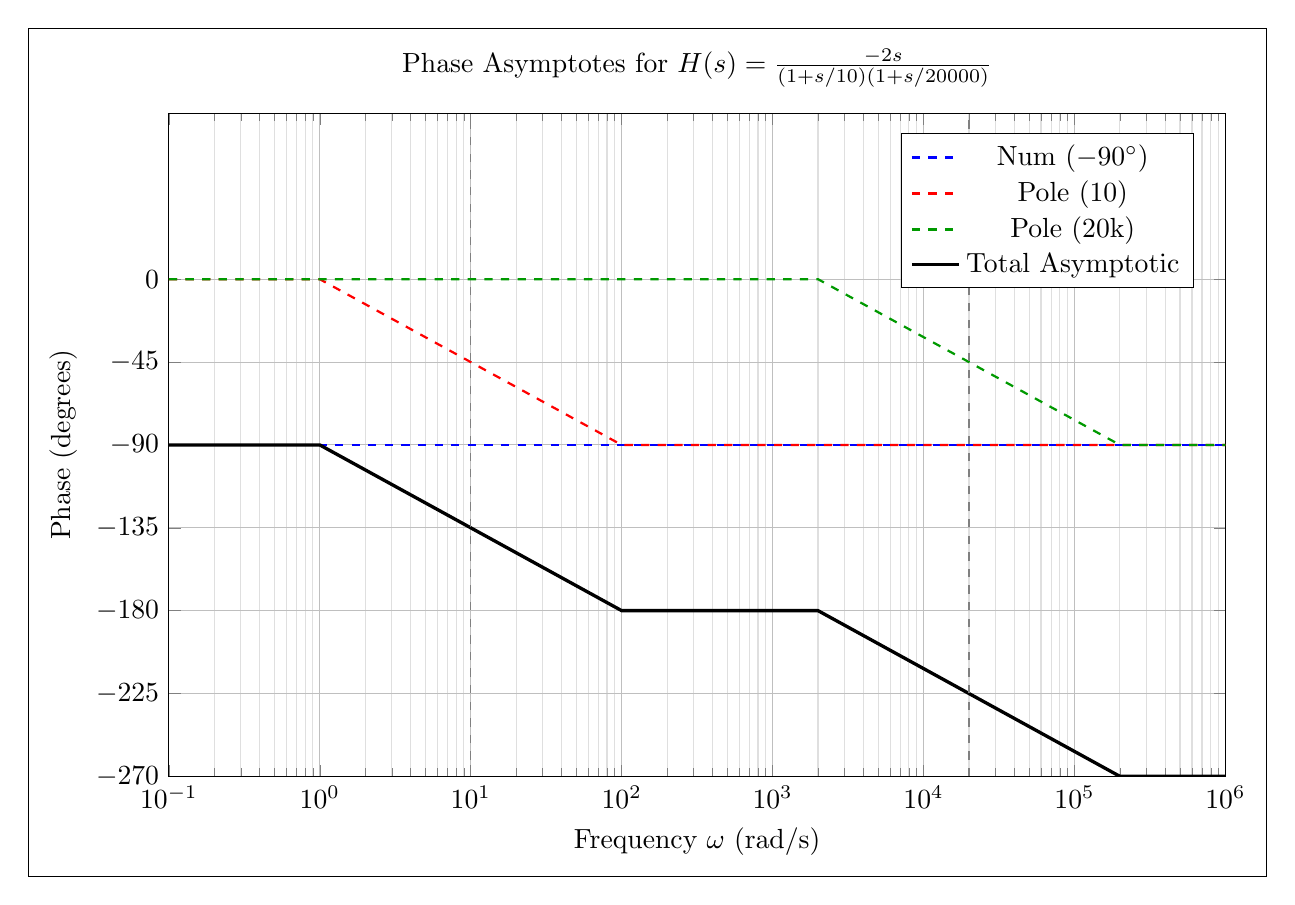
\begin{tikzpicture}[show background rectangle]
    \begin{semilogxaxis}[
        width=15cm, height=10cm,
        title={Phase Asymptotes for $H(s) = \frac{-2s}{(1+s/10)(1+s/20000)}$},
        xlabel={Frequency $\omega$ (rad/s)},
        ylabel={Phase (degrees)},
        grid=both,
        xmin=0.1, xmax=1000000,
        ymin=-270, ymax=90,
        minor grid style={gray!25},
        major grid style={gray!50},
        legend pos=north east,
        ytick={0, -45, -90, -135, -180, -225, -270},
    ]

    % 1. Numerator: -2s => -90 degrees constant
    \addplot[blue, thick, dashed, domain=0.1:1000000] {-90};
    \addlegendentry{Num ($-90^\circ$)}

    % 2. Pole at 10 => 0 until 1, then down to -90 at 100
    \addplot[red, thick, dashed] coordinates {
        (0.1, 0) (1, 0) (100, -90) (1000000, -90)
    };
    \addlegendentry{Pole ($10$)}

    % 3. Pole at 20000 => 0 until 2000, then down to -90 at 200000
    \addplot[green!60!black, thick, dashed] coordinates {
        (0.1, 0) (2000, 0) (200000, -90) (1000000, -90)
    };
    \addlegendentry{Pole ($20\text{k}$)}

    % Total Asymptotic Phase (Sum)
    \addplot[black, very thick] coordinates {
        (0.1, -90)          % Initial sum: -90 + 0 + 0 = -90
        (1, -90)            % Pole 1 starts breaking at 1
        (100, -180)         % Pole 1 finishes breaking at 100 (-90-90=-180). Pole 2 hasn't started (2000).
        (2000, -180)        % Pole 2 starts breaking at 2000
        (200000, -270)      % Pole 2 finishes breaking at 200000 (-180-90=-270)
        (1000000, -270)
    };
    \addlegendentry{Total Asymptotic}

    % Break frequency markers
    \draw[dashed, gray] (axis cs:10, -270) -- (axis cs:10, 90);
    \draw[dashed, gray] (axis cs:20000, -270) -- (axis cs:20000, 90);
    
    \end{semilogxaxis}
\end{tikzpicture}
\end{document}
